\documentclass[%
	11pt,
	a4paper,
	utf8,
	%twocolumn
		]{article}	

\usepackage{style_packages/podvoyskiy_article_extended}


\begin{document}
\title{Общие и специальные вопросы оптимизации}

\author{\itshape Подвойский А.О.}

\date{}
\maketitle

\thispagestyle{fancy}

%Здесь приводятся заметки по специальным вопросам теории оптимизации


\shorttableofcontents{Краткое содержание}{1}

\tableofcontents

\section{Полезные ссылки}

\url{https://github.com/ceandrade/brkga_mip_feasibility}

\section{Конспект статьи Gamrath, G. Structure-driven fix-and-propagate heuristics ofr MIP}

DINS, RINS, RENS, Crossover и Analytic Center Search определяют свои окрестности с помощью фиксации переменных. LNS-эвристики, базирующиеся на приеме фиксации переменных, страдают от внутренних конфликтов: исходное пространство поиска должно быть значительно сжато (reduced); таким образом, приходится фиксировать большое количество переменных. Но при этом, чем больше переменных фиксируется, тем выше вероятность, что подпроблема не содержит улучшающего решения или вообще дает недопустимое решение.

\emph{Клика} (clique) -- это множество $ \mathcal{C} $ бинарных переменных, в котором не более чем одна переменная может быть выставлена в \emph{единицу}. Клика может быть представлена как линейное неравенство $ \sum_{i \in \mathcal{C}} x_i \leqslant 1 $.

По аналогии \emph{обращенная клика} (negated clique) -- это множество бинарных переменных, в котором не более чем одна переменная может быть выставлена в \emph{ноль}.

В современных MIP-решателях множества выявляенных клик собираются в так называемую \emph{таблицу клик} (clique table). Эта таблица используется компонентами решателя, например, для создания секущих (cuts) или для построения более интенсивного снижения размерности задачи на шаге пресолвинга и распространения.

\emph{Блокировки переменных} (variable locks) определяются непосредственно по матрице ограничений и показывают сколько ограничений могут быть заблокированы при увеличении или уменьшении значения переменной. В случае MIP с $ \leqslant $-ограничениями число $ \xi_i^{+} $ \emph{верхних блокировок} (up-locks) переменной $ x_i $ -- это число ограничений, в которых эта переменная имеет положительный коэффициент $ a_{ri} $. А число $ \xi_i^{-} $ \emph{нижних блокировок} (down-locks) -- это число ограничений с отрицательным значением коэффициента переменной.

The cliuqe-driven-fix-and-propagate heuristic. Если положить только одну бинарную переменную равной единице, то распространение домена зафиксирует оставшиеся бинарные переменные клики в 0, но кроме это еще и применит много различных изменений домена, сообразно соответствующим переменным. Выбирая для фиксации в единицу самую <<дешевую>> переменную, т.е. переменную с наименьшим коэффициентом в целевой функции, мы стремимся получить решение с низким значением целевой функции.

Важно: поиск новых существующих решений часто наиболее эффективен в коренвом узле, когда первичная эвристика может непосредственно привести к глобальным фиксациям, более жестким секущим (tighter cutting planes) и лучшим начальным решениям о ветвлении.


\section{Конспект диссертации Ахтерберга по CIP}

\subsection{Mixed Integer Programs}

Задачи SAT относятся к классу \emph{NP-полных}, а BP, IP и MIP -- к классу \emph{NP-трудных} \cite[\strbook{11}]{achterberg:constr_int_prog}.

\section{Методы решения задач линейного программирования}

Задачи линейного программирования относятся к подклассу задач выпуклого программирования \cite[\strbook{57}]{vorontsova:convex_opt-2021}.

\subsection{Симплекс-метод Данцига}

Симплекс-метод Данцига предназначен для решения задач линейного программирования в релаксированной постановке (то есть без учета ограничений на целочисленность переменных) \cite[\strbook{13}]{achterberg:constr_int_prog}.

\remark{
	В худшем случае симплекс-метод работает за экспоненциальное время, но в целом на практике обычно он работает очень быстро, и многочисленные эксперименты и исследования метода подтвердили полиномиальное время работы \cite[\strbook{61}]{vorontsova:convex_opt-2021}
}

Для оценки вычислительной сложности симплекс-метода Данцига Спилман и Тенг предложили использовать \emph{сглаженный анализ}. Сглаженный анализ -- вероятностный анализ алгоритма, при котором изучается работа алгоритма при незначительном случайном возмущеннии конкретных входных данных, а затем ищется зависимость производительности алгоритма от размера входа и от среднеквадратичного отклоненеия возмощений.

Так вот Спилман и Тенг показали, что симплекс-метод имеет \emph{\underline{полиномиальную} сглаженную сложность}\footnote{В том же 2006 году оценка симплекс-метода Спилмана и Тенга была улучшена. Р. Вершининым. Он показал, что ожидаемое время работы симплекс-метода на незначительно измененных входных данных является полиномом от логарифма количества ограничений $ n $}. Эти результаты означают, что хотя и существуют задачи, на которых симплекс-метод будет работать \emph{экспоненциально} долго, но если исходные данные таких задач (коэффициенты целевой функции и ограничений) подвергнуть незначительному изменению, то с достаточно высокой вероятностью симплекс-метод на возмущенной задаче уже будет работать за \emph{полиномиальное время} \cite[\strbook{62}]{vorontsova:convex_opt-2021}.

В конце 1970-х годов обнаружили, что алгоритмы, в общем случае решающие задачи линейного программирования за полиномиальное время, все-таки существуют. Все такие полиномиальные алгоритмы -- \emph{методы внутренней точки} (первый метод внутреней точки с полиномиальной сложностью -- метод Кармаркара) и \emph{метод эллипсоидов} -- отличались от симплекс-метода геометрическим подходом.

В течение 50 лет оставался открытым вопрос, существует ли полиномиальный алгоритм, который работает подобно симплекс-методу, перебирая только вершины (угловые точки) допустимого множества задачи. Ответ на этот вопрос дали Келнер и Спилман в 2006 году: они представили \underline{рандомизированный} симплекс-метод с \emph{полиномиальным временем работы}.

\remark{%
В современных оптимизационных пакетах задачи линейного программирования средней размерности (вплоть до сотен тысяч и даже миллиона переменных или ограничений) решаются \underline{\itshape методами внутренней точки}.
}

Постановка задачи. Найти максимум функции
\begin{align*}
f(x) = \sum_{j=1}^{n} c_j x_j \leftarrow c^T x
\end{align*}
при ограничениях
\begin{align*}
	\sum_{j=1}^{n} a_{ij} x_j = b_i, \ i = 1, \ldots, m\  (m < n) \leftarrow Ax = b,\\
	x_j \geqslant 0, \ j = 1, \ldots, n.
\end{align*}

Такая постановка называется \emph{канонической}, а искомое решение $ x^{*} = (x_1^{*}, \ldots, x_n^{*})^T $ -- \emph{оптимальным}.

Замечания:
\begin{itemize}
	\item Максимизируемая функция и ограничения \underline{линейны} по $ x_j, \ j = 1, \ldots, n $,
	
	\item Задача содержит ограничения на неотрицательность переменных, присутствие которых диктуется процедурой симплекс-метода. Если по физической постановке задачи какая-либо переменная, например, $ x_n $, неограничена по знаку, то ее можно представить в виде $ x_n = x_{n+1} - x_{n+2} $, где $ x_{n+1}, x_{n+2} \geqslant 0 $,
	
	\item В ограничениях $ \sum\limits_{j=1}^{n} a_{ij} x_j = b_i, \ i = 1, \ldots, m\  (m < n) $ будем считать переменные $ b_i \geqslant 0, \ i = 1, \ldots, m $.
\end{itemize}

Стратегия метода Данцига решения описаной задачи основана на особенностях постановки этой задачи. Множество
\begin{align*}
	X = \{ x \, | \, \sum_{i}^{n} a_{ij} x_j = b_i, \ i = 1, \ldots, m, \ x \in \mathbb{R}^n, \ x_j \geqslant 0, \ j = 1, \ldots, n \}
\end{align*}
допустимых решений задачи -- есть выпуклое множество, которое геометрически представляет собой \emph{выпуклый политоп}\footnote{Политоп -- подмножество Евклидова пространства, представимое объединением симплексов ($ n $-мерное обобщение треугольника)}, имеющий конечное число \emph{крайних точек}.

\emph{Крайней точкой выпуклого множества} $ X $ называется точка $ x \in X $, которая не может быть выражена в виде выпуклой комбинации других точек $ y \in X, x \neq y $.

Стратегия решения задачи симплекс-методом состоит в направленном переборе базисных решений, определяющих крайние точки политопа. Направленность перебора предполагает следующую организацию вычислительного процесса \cite{panteleev}:
\begin{enumerate}
	\item Нахождение базисного решения (метод Гаусса-Жордана, переход к $ M $-задаче),
	
	\item Переход от одного базисного решения к другому таким образом, чтобы обеспечить улучшение целевой функции (другими словами, переход от одной \emph{вершины политопа} к другой в направлении улучшения целевой функции).
\end{enumerate}

\subsection{Двойственный симплекс-метод}

Теорема двойственности подсказывает, что симплекм-метод, примененный к двойственной задаче, может дать и решение прямой задачи (по крайней мере, если обе ЗЛП имеют допустимые векторы). Различные реализцаии этой идеи приводят к семейству процедур, объединяемых под названием <<двойственный симплекс-метод>>. 

\subsection{Метод барьеров (метод внутренней точки)}

\emph{Метод барьеров} (также называемый \emph{методом внутренней точки} или \emph{методом внутренних штрафов}) является методом решения условных задач оптимизации с ограничениями вида неравенств
\begin{align*}
	\min\limits_x f(x), \qquad g_i(x) \leqslant 0, \ i = 1, \ldots, m,
\end{align*}
где $ f, g_1, \ldots, g_m:\mathbb{R}^n \rightarrow \mathbb{R} $ -- дважды непрерывно дифференцируемые функции, $ x \in \mathbb{R}^n $ -- целевая переменная.

Основная идея метода барьеров заключается в сведении \emph{исходной \underline{условной} задачи} к последовательности специальным образом построенных \emph{\underline{безусловных} задач}, решения которых сходятся к решению исходной \underline{условной} задачи. Это делается с помощью барьерной функции.

Пусть $ Q $ -- множество, задаваемое функциональными ограничениями $ g_1, \ldots, g_m $
\begin{align*}
	Q := \{ x \in \mathbb{R}^n: g_i (x) \leqslant 0 \quad \forall \ 1 \leqslant i \leqslant m \}.
\end{align*}

\emph{Барьерной функцией} (или \emph{функцией внутренних шрафов}) для множества $ Q $ называется любая функция $ F: \text{int} \, Q \rightarrow \mathbb{R} $, определенная на внутренности множества $ Q $ и являющаяся достаточно гладкой, которая обладает барьерным свойством: $ F(x) \rightarrow + \infty $ при приближении $ x $ к границе множества $ Q $ изнутри.

Имея в распоряжении барьерную функцию, определим для каждого $ t \geqslant 0 $ вспомогательную функцию $ f_t: \text{int} \, Q \rightarrow \mathbb{R} $ по формуле
\begin{align*}
	f_t(x) := t f(x) + F(x)
\end{align*}

Оказывается, что при $ t \rightarrow + \infty $ точка $ x^{*}(t) $ сходится ко множеству решений исходной условной задачи. Обозначим $ x^{*}(t) := \argmin_{ x \in \text{int} Q } f_t(x) $. Множество точек $ \{ x^{*}(t): t \geqslant 0 \} $ называется \emph{центральным путем}.

{\color{blue}Общая схема метода барьеров}:
\begin{enumerate}
	\item Выбрать начальное приближение $ x_0 \in \text{int} \, Q $ и начальный параметр $ t_0 > 0 $.
	
	\item На каждой итерации $ k \geqslant 0 $:
	\begin{enumerate}
		\item Вычислить точку 
\begin{align*}
x_{k+1} := \argmin_{ y \in \text{int} Q } f_{t_k} (y),
\end{align*}
    используя некоторый \emph{метод \underline{безусловной} оптимизации} с начальной точкой $ x_k $.
    
    \item Увеличить параметр $ t $: выбрать $ t_{k+1} > t_k $ (чтобы в итоге $ t_k \rightarrow + \infty $)
	\end{enumerate}
\end{enumerate}

Заметим, что задача оптимизации, возникающая на каждой итерации метода барьеров в реальности является <<\emph{безусловной}>>, несмотря на присутствие в этой задаче условия $ x \in \text{int} Q $. Действительно, за счет барьерного свойства\footnote{Вернее за счет барьерного свойства барьерной функции} целевая функция $ f_t $ стремится к $ + \infty $ при приближении к границе множества $ Q $, поэтому никакой <<разумный>> метод оптимизации достаточно близко к границе множества $ Q $ никогда не подойдет, и, с точки зрения самого метода, целевая функция как бы задана всюду. Тем не менее, здесь необходима определенная аккуратность.

Например, пусть для решения вспомогательной задачи (задача безусловной оптимизации) используется метод спуска: сначала $ y_0 = x_k $, далее на каждой итерации $ l \geqslant 0 $ строится направление спуска $ d_l \in \mathbb{R}^n $ для функции $ f_{t_k} $ в точке $ y_l $, и выполняется шаг
\begin{align*}
	y_{l + 1} := y_l + \alpha_l d_l,
\end{align*}
где $ \alpha_l \geqslant 0 $ -- длина шагов. Поскольку метод барьеров по построению всегда работает с внутренними точками множества $ Q $ (отсюда и альтернативное название), то для всех достаточно маленьких длин шагов $ \alpha_l $ новая точка $ y_{l+1} $ будет принадлежать множеству $ Q $, а значение функции $ f_{t_k} $ в этой точке уменьшится по сравнению с текущей точкой $ y_l $. Однако, если длина шага $ \alpha_l $ выбрана слишком большой, то точка $ y_{l+1} $ может вообще оказаться за пределами множества $ Q $ -- такое вполне может произойти при подборе шага в стандартном алгоритме линейного поиска. Чтобы избежать этой проблемы, стандартную процедуру линейного поиска необходимо модифицировать -- запретить ей вычислять функцию в точках за пределами множества $ Q $.

\subsubsection{Полная спецификация метода барьеров}

Несмотря на то, что гипотетически в методе барьеров можно использовать \emph{любую} комбинацию \emph{барьерной функции} и \emph{метода безусловной оптимизации}, наиболее эффективной (как с точки зрения теория, так и практики) оказывается связка \emph{\underline{логарифмического барьера}} и \emph{\underline{метода Ньютона}} (имеет локальную квадратичную сходимость).

Логарифмический барьер в общем виде имеет вид
\begin{align*}
	F(x) := - \sum_{i=1}^m \ln (- g_i(x))
\end{align*}

В модели LASSO, как и в любой модели линейной регрессии, прогнозирование выполняется с помощью линейной комбинации компонент вектора $ a $ (вектор признаков) с некоторыми фиксированными коэффициентами $ x \in \mathbb{R}^n $ (это параметры модели)
\begin{align*}
	b(a) := \left< a, x \right>
\end{align*}

Коэффициенты $ x $ (параметры модели) настраиваются с помощью решения следующей оптимизационной задачи
\begin{align}\label{eq:lasso}
	\varphi(x) := \dfrac{1}{2} \sum_{i=1}^{m} (\left< a_i, x \right> - b_i)^2 + \lambda \sum_{j=1}^{n} | x_j | := \dfrac{1}{2} \| A x - b \|_2^2 + \lambda \| x \|_1 \rightarrow \min_{ x \in \mathbb{R}^n }
\end{align}

Здесь $ \lambda > 0 $ -- коэффициент регуляризации (параметр модели). Особенностью LASSO является использование имеено $ l_1 $-регуляризации. Такая регуляризация позволяет получить разреженное решение. В разреженном решении $ x^{*} $ часть компонент равна нулю. Нулевые веса соответствуют исключению соответствующих признаков из модели (признание их неинформативности).

Двойственной задачей к  задаче \eqref{eq:lasso} является
\begin{align*}\label{eq:dual_lasso}
	\max_{ \mu \in \mathbb{R}^n } \big[ - \dfrac{1}{2} \| \mu \|_2^2 - \left< b, \mu \right>: \| A^T \mu \|_{\infty} \leqslant \lambda \,\big]
\end{align*}

Таким образом, имея в распоряжении допустимую двойственную точку $ \mu \in \mathbb{R}^n $, т.е. такую что $ \| A^T \mu \|_{\infty} \leqslant \lambda $, можно вычислить следующую оценку для невязки в этой задаче
\begin{align}
	\varphi (x) - \varphi^{*} \leqslant \dfrac{1}{2} \| Ax - b \|_2^2 + \lambda \| x \|_1 + \dfrac{1}{2} \| \mu \|_2^2 + \left< b, \mu \right> =: \eta(x, \mu)
\end{align}

Величина $ \eta{(x, \mu)} $ называется зазором двойственности и обращается в ноль в оптимальных решениях ($ x^{*} $ и $ \mu^{*} $ задач \eqref{eq:lasso} и \eqref{eq:dual_lasso}). Заметим, что решения $ x^{*} $ и $ \mu^{*} $ связаны между собой следующим соотношением: $ A x^{*} - b = \mu^{*} $. 

Поэтому для фиксированного $ x $ естественным выбором соответствующего $ \mu $ будет
\begin{align*}
	\mu(x) := \min \Bigg(1, \dfrac{\lambda}{ \| A^T (A x - b) \|_{\infty} } \Bigg) (Ax - b)
\end{align*}

Такой выбор обеспечивает стремление зазора двойственности $ \eta(x, \mu(x)) $ к нулю при $ x \rightarrow x^{*} $, что позволяет использовать условие $ \eta (x, \mu(x)) < \varepsilon $ в качестве критерия остановки в любом итерационном методе решения задачи \eqref{eq:lasso}.

Выполнив эквивалентное преобразование задачи через надграфик, задачу \eqref{eq:lasso} можно переписать в виде гладкой условной задачи
\begin{align*}
	\min_{x, u} \bigg( \dfrac{1}{2} \| Ax - b\|_2^2 + \lambda \left< 1_n, u \right> \bigg) \qquad x \preceq u, \ x \succeq - u,
\end{align*}
где $ x, u \in \mathbb{R}^n $ и $ 1_n := (1, \ldots, 1) \in \mathbb{R}^n $. Эта задача является задачей квадратичного программирования, и ее можно решать методом барьеров.


\section{Методы решения задач линейного целочисленного программирования}

\subsection{Общие положения}

В случае метода ветвей-и-границ, основанного на решении задачи линейного программирования (LP-based Branch-and-Bound for MIP) порядок действий следующий:
\begin{itemize}
	\item Сначала мы решаем ихсодную задачу линейного программирования (original problem) в релаксированной постановке (LP relaxation). Результатом может быть
	\begin{enumerate}
		\item задача линейного программирования (LP) неограничена (unbounded), следовательно задача линейного программирования в частично-целочисленной постановке (MIP) либо тоже неограничена, либо недопустима (infeasible)
		
		\item LP недопустима, следовательно недопустима и MIP
		
		\item получено допустимое решение MIP, следовательно это оптимальное решение для MIP
		
		\item получено оптимальное решение для LP, которое является недопустимым для MIP
	\end{enumerate}
\end{itemize}

В первых трех случаях мы заканчиваем. В последнем случае мы должны ветвиться.

\remark{
  Ключ к успеху останавливаться рано и часто. Другими словами, надо уметь быстро идентифицировать потенциально слабое решение и не тратить на него много времени
}

Замечание об эвристиках:
\begin{itemize}
	\item Решение задачи линейного программирования в релаксированной постановке может интерпретироваться как эвристика. Часто не способна найти допустимое решение
	
	\item Rounding/Diving:
	\begin{itemize}
		\item Rounding: Округляет нецелочисленные значения целочисленных переменных,
		
		\item Diving: фиксирует только одну целочисленную переменную, решает LP
	\end{itemize}

    \item Метаэвристики -- имитация отжига, поиск Табу, генетические алгоритмы и пр.
    
    \item Optimization-based эвристики:
    \begin{itemize}
    	\item RINS, локальное ветвление
    \end{itemize}

    \item Доменно-ориентированные эвристики. Часто оказываются очень полезны
\end{itemize}

Один из способов снизить временные издержки заключается в том, чтобы постараться сделать дерево поиска как можно более компактным

Стратегия ветвления (Branching Rule) очень важна.

Strong Branching на самом деле решает LP задачу в релаксированной постановке для каждой подпроблемы для каждой потенциальной переменной ветвления. Pseudo-costs приближает изменения границы на основе предыдущей информации, собранной при построении дерева ветвей-и-границ.

Эвристики округления \cite{berthold:primal_heur_scip}:
\begin{itemize}
	\item Simple Rounding: всегда возвращает допустимое решение,
	
	\item Rounding: может нарушать ограничения,
	
	\item Shifting: может <<освобождать>> (unfix) целочисленные переменные,
	
	\item Integer Shifting: решает LP-задачу.
\end{itemize}

\emph{Алгоритм RENS} -- An LNS (Large Neighborhood Search) Rouding Heuristic:
\begin{enumerate}
	\item $ \bar{x} $ $\leftarrow$ оптимальное решение задачи в релаксированной постановке,
	
	\item Фиксирует все целочисленные переменные,
	
	\item Урезает область,
	
	\item Решает получившуюся подпроблему MIP.
\end{enumerate}

\emph{Алгоритм Feasibility Pump} (Fischetti, Lodi et al.):
\begin{enumerate}
	\item Решаем LP-задачу
	
	\item Округляем оптимальное решение LP-задачи
	
	\item Если полученное решение допустимо, останавливаемся. В противном случае изменяем цель и возвращаемся к пункту 1
\end{enumerate}

Советы:
\begin{itemize}
	\item Использовать ограничения (limits) для снижения размерности задачи,
	
	\item Diving: стараться использовать округление на лету,
	
	\item Отадавать предпочтение бинарным переменным перед целочисленными. 
\end{itemize}

\subsection{Метод ветвей и границ}

Постановка задачи (Mixed Integer Linear Programming, MILP)
\begin{align*}
	f(x) = \sum_{j=1}^{n} c_j x_j \rightarrow \max
\end{align*}
при ограничениях
\begin{align*}
	\sum_{j=1}^{n} a_{ij} x_j \geqslant b_i, \ i = 1, \ldots, m,\\
	x_j \geqslant 0, \ x \in \mathbb{Z}, \ j = 1, \ldots, n.
\end{align*}

\remark{%
Описанная задача является задачей линейного целочисленного программирования. Ограничения, связанные с целочисленностью, могут быть наложены не на все переменные, а лишь на их часть
}

\textbf{Стратегия поиска}

Для корня дерева ветвей-и-границ (branch-and-bound tree) описанная задача решается \emph{симплекс-методом} \underline{без учета ограничений на целочисленность} (т.е. в релаксированной постановке). Считаеся, что она имеет решение. На полученном оптимальном решении $ x^{0*} = (x_1^{0*}, \ldots, x_n^{0*}) $ вычисляется значение \emph{целевой функции} $ f(x^{0*}) $.

Если решение $ x^{0*} $ является целочисленным, то поставленная задача решена. Если решение $ x^{0*} $ оказывается \underline{нецелочисленным}, то значение $ f(x^{0*}) $ (полученное для решаемой задачи в релаксированной постановке) является \emph{верхней границей} (потому что мы решаем задачу на максимум) возможных оптимальных значений $ f(x) $ на целочисленных решениях.

При нецелочисленном решении дальнейшая процедура решения задачи состоит в ее ветвлении на две подзадачи. Целью этого ветвления является разбиение множества допустимых решений на два подмножества путем построения дополнительных ограничений таким образом, чтобы исключить нецелочисленную точку $ x^{0*} $ и сделать решение по крайней мере одной из задач целочисленным по одной выбранной координате $ x_k $.

Координатой $ x_k $ может быть \cite[\strbook{339}]{panteleev}:
\begin{enumerate}
	\item Нецелочисленная координата с наименьшим или наибольшим индексом.
	
	\item Нецелочисленная координата с наименьшей или наибольшей дробной частью.
	
	\item Нецелочисленная координата, которой соответствует наибольший коэффициент в целевой функции.
	
	\item Нецелочисленная координата, выбранная на основани приоритетов, определяемых физическим содержанием задачи.
\end{enumerate}

Для построения дополнительных ограничений округляем нецелочисленное решение вниз и исследуем область значений левее, т.е. $ x_k \leqslant \floor{x_k^{0*}} $, и округляем вверх и исследуем область правее, т.е. $ \ceil{x_k^{0*}} \leqslant x_k $.

Построение дополнительных ограничений позволило исключить из рассмотрения оптимальное \underline{нецелочисленное} решение $ x^{0*} $ и обеспечить \underline{целочисленность} значений координаты $ x_k $.

\begin{figure}[h]
	\centering
	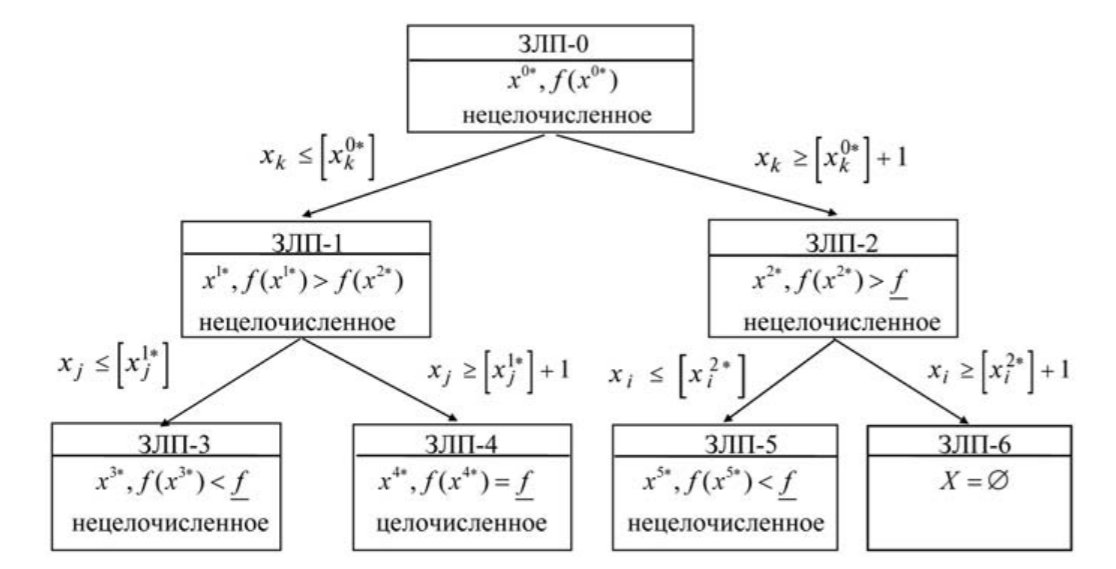
\includegraphics[scale=0.7]{figures/bb_tree.png}
	\caption{ Пример дерева ветвей-и-границ }\label{fig:bb_tree}
\end{figure}

Задачи ЗЛП-1 и ЗЛП-2 записываются в виде, изображенном на \pic{fig:zlp_1_and_zlp_2}.

\begin{figure}[h]
	\centering
	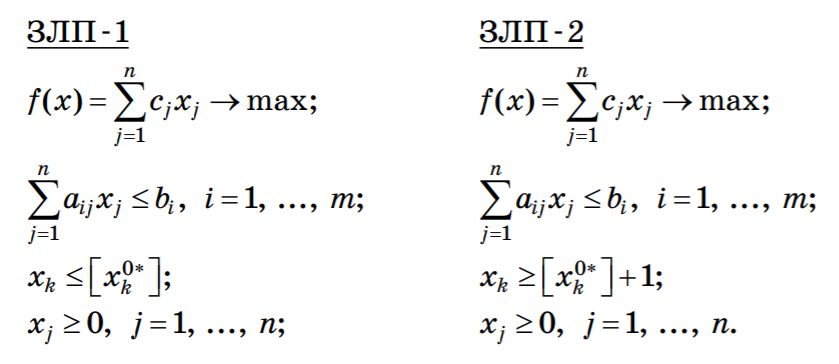
\includegraphics[scale=0.6]{figures/zlp_1_and_zlp_2.png}
	\caption{ Подзадачи корневого узла дерева ветвей-и-границ }\label{fig:zlp_1_and_zlp_2}
\end{figure}

Задачи ЗЛП-1 и ЗЛП-2 решаются самостоятельно симплекс-методом \emph{без учета ограничений на целочисленность} координта $ x_j, \ j = 1, \ldots, n $. Вычисляются значения функции $ f(x) $ на оптимальных решениях обеих задач. Если ни одна из них не имеет целочисленного решения, то выбрирается задача для приоритетного дальнейшего ветвления по установленному правилу: например, приоритетному ветвлению подлежит та задача, в которой значение $ f(x) $ на оптимальном \emph{нецелочисленном} решении максимально.

Пусть $ f(x^{1*}) > f(x^{2*}) $, тогда задача ЗЛП-1 первой ветвится на ЗЛП-3 и ЗЛП-4, которые решаются симплекс-методом \emph{без учета требований на целочисленность} с последующим анализом решений \cite[\strbook{340}]{panteleev}. Если ни одна из задач ЗЛП-3 и ЗЛП-4 не имеет целочисленного решения, приступают к ветвлению задачи ЗЛП-2.

Процесс ветвления продолжается до тех пор, пока не будет получено в одной из ветвей целочисленное решение. Пусть задача ЗЛП-4 имеет целочисленное решение.  Обозначим $ \underline{f} $ -- значение функции на первом целочисленном решении: $ \underline{f} = f(x^{4*}) $. Соответсвующее целочисленное решение включается в множество $ \bar{X}^* $ возможных оптимальных решений исходной задачи.

После того, как найдено первое целочисленное решение, вопрос о дальнейшем ветвлении других задач решается на основании сравнения значений $ f(x^{k*}) $ на оптимальных \underline{нецелочисленных} решениях в оставшихся ветвях со значением $ \underline{f} $.

Если $ f(x^{k*}) \leqslant \underline{f} $ для всех оставшихся $ k $, то расчет закончен. Решениями исходной задачи являются те целочисленные решения $ x^{k*} $, для которых $ f(x^{k*}) = \underline{f} $.

Если $ f(x^{k*}) > \underline{f} $, то соответствующая этому номеру $ k $ задача ветвится далее. Так, на \pic{fig:bb_tree} имеем $ f(x^{2*}) > \underline{f} $ и $ f(x^{3*}) < \underline{f} $. Задача ЗЛП-2 подлежит ветвлению на ЗЛП-5, ЗЛП-6, а задача ЗЛП-3 не подлежит. Задача ЗЛП-6 не имеет решения, так как множество допустимых решений пустое, и далее не рассматривается. Задача ЗЛП-5 имеет нецелочисленное решение $ x^{5*}, f(x^{5*}) $. Если $ f(x^{5*}) < \underline{f} $, то решение задачи закончено и $ x^* = x^{4*}, f(x^*) = \underline{f} $. В противном случае задача ЗЛП-5 ветвится дальше.

Если в одной из задач получено целочисленное решение, то ее ветвление далее не прозводится. Если соответствующее значение целевой функции $ \geqslant \underline{f} $, решение считается принадлежащим множеству $ X^* $ возможных оптимальных решений исходной задачи.

Если значение целевой функции $ < \underline{f} $, целочисленное решение не включается в множество $ X^* $.

Таким образом, ветвление какой-либо задачи заканчивается, если выполняется одно из условий \cite{panteleev}:
\begin{enumerate}
	\item решение целочисленное,
	
	\item значение целевой функции данной задачи $ \leqslant \underline{f} $,
	
	\item множество допустимых решений пустое.
\end{enumerate}

Если ветвление всех задач закончено, то в множестве $ X^* $ выбирается решение (решения), которому соответствует наибольшее значение целевой функции. Оно является решением исходной задачи. Если множество $ X^* $ пустое, то исходная задача не имеет решения.

\subsection{Пресолверы, пропагаторы и прайсеры}

Пресолвинг предназначен для:
\begin{itemize}
	\item снижения размерности задачи,
	
	\item усиливания релаксации LP-задачи,
	
	\item повышения численной стабильности релаксации LP-задачи,
	
	\item извлечения полезной информации.
\end{itemize}

Пропагаторы предназначены для:
\begin{itemize}
	\item локального упрощения модели,
	
	\item улучшения двойственной границы,
	
	\item обнаружения недопустимых решений.
\end{itemize}

Прайсеры (pricing) предназначены для:
\begin{itemize}
	\item поиска переменных с отрицательными сниженными потерями (negative reduced costs) или доказательства отсутствия последних,
	
	\item динамического старения переменных,
	
	\item 
\end{itemize}



\subsection{Первичные эвристики в SCIP}

Алгоритм ветвей-и-границ представляет собой \emph{полную} (complete) процедуру. Это означает, что алгоритм гарантирует оптимальное решение каждой проблемы за конечное время. Однако, это очень дорогой в вычислительном смысле метод и в худшем случае временные издержки будут экспоненйиально зависеть от размерности задачи.

В противоположенность первичные эвристики относятся к \emph{неполным} (incomplete) методам. То есть они пытаются найти допустимое решение приемлемого качества за небольшой промежуток времени. Но они не гарантируют оптимальности решения.

Первичные эвристики в SCIP условно могут быть разделены на 4 категории \cite{achterberg:constr_int_prog}:
\begin{itemize}
	\item Эвристики округления (rounding heuristics) пытаются округлять значения переменных релаксированного решения таким образом, чтобы полученное округленное решение оставалось допустимым,
	
	\item Глубокие эвристики (diving heurisctics) начинают с текущего релаксированного решения задачи и итеративно фиксируют целочисленные значения целочисленных переменных и решают текующую задачу заново,
	
	\item Целевые глубокие эвристики (objective diving heuristics) похожи на глубокие эвристики, но вместо фиксации переменных, они изменяют значения коэффициентов в целевой функции,
	
	\item Улучшающие эвристики (improvenment heuristics) исследуют одно и несколько допустимых решений и пытаются построить такое решение, которому отвечает более низкое (в случае задачи минимизации) или более высокое (в случае задачи максимизации) значение целевой функции.
\end{itemize}

\subsubsection{Эвристики округления}

\paragraph{RENS} 


\section{Общие положения постановки частично-целочисленного линейного программирования}

Задача линейного программирования в частично-целочисленной постановке (Mixed Integer Linear Program, MILP, MIP) записывается в форме
\begin{align*}
	\min c^T x,\\
	Ax = b,\\
	x \geqslant 0,\\
	x_i \in \mathbb{Z} \quad \forall i \in \mathcal{I}
\end{align*}

Задача, когда все переменные являются целочисленными, называется задачей линейного программирования в чистой целочисленной постановке (Pure Integer Linear Program, ILP, IP).

Если все переменные принимаются значения из множества $ \{ 0, 1 \} $, то задача называется задачей линейного программирования 0-1 (0-1 linear program).

Включение целочисленных переменных в постановку задачи расширяет возможности моделирования.

Задачи линейного программирования могут быть решены за полиномиальное время \emph{методами внутренней точки} (метод эллипсоида, алгоритм Кармаркара). 

Задачи целочисленного программирования относятся к классу NP-трудных:
\begin{itemize}
	\item на текущий момент не известны алгоритмы, способные решить этот такого рода задачи за полиномиальное время,
	
	\item И, вообще говоря, есть мало шансов, что такие алгоритмы когда-нибудь будут найдены.
\end{itemize}

Релаксированное решение можно получить, сняв ограничения на целочисленность
\begin{align*}
	\min c^T x,\\
	Ax = b,\\
	x \geqslant 0.
\end{align*}

\remark{
Задачу линейного программирования в частично-целочисленной постановке нельзя решить, просто перейдя от решения задачи в релаксированной постановке с последующем округлением переменных
}

Например, оптимальным решением задачи линейного программирования в чистой целочисленной постановке будет
\begin{align*}
	\max x + y\\
	-2x + 2 y \geqslant 1,\\
	-8 x + 10 y \leqslant 13,\\
	x,y \geqslant 0,\\
	x,y \in \mathbb{Z}
\end{align*}
вектор $ (x, y) = (1, 2) $, которому отвечает целевая функция со значением 3.

А релаксированным оптимальным решением будет вектор $ (x, y) = (4, 4.5) $ со значением целевой функции 9.5. 

Не существует прямого способа перейти от релаксированного решения к целочисленному.

\begin{figure}[h]
	\centering
	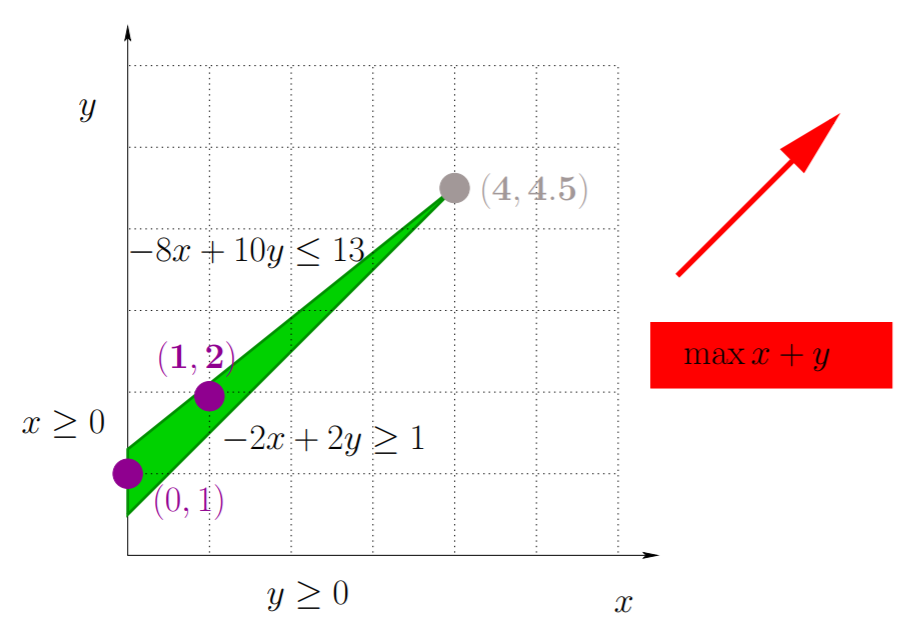
\includegraphics[scale=0.55]{figures/lp_and_mip.png}
	\caption{ Связь релаксированной и целочисленной постановок задачи }\label{fig:lp_and_mip}
\end{figure}

Предполагается, что переменные ограничены, т.е. имеют нижнюю и верхнюю границы.

Через $ P_0 $ обозначим рассматриваемую постановку задачи, а через $ LP(P_0) $ релаксированное решение задачи $ P_0 $. Если в оптимальном релаксированном решении $ LP(P_0) $ все целочисленные переменные принимают целочисленные значения, то это решение будет решением исходной задачи $ P_0 $.

В противном случае для целочисленной переменной $ x_j $, которая принимает нецелочисленное значение $ \beta_j, \ \beta_j \notin \mathbb{Z} $ в оптимальном релаксированном решении $ LP(P_0) $, определяются подзадачи
\begin{align*}
	P_1 := P_0 \wedge x_j \leqslant \floor*{\beta_j},\\
	P_2 := P_0 \wedge x_j \geqslant \ceil*{\beta_j}.
\end{align*}

Тогда физичным решением исходной задачи будет
$$
feasibleSols(P_0) = feasibleSols(P_1) \cup feasibleSols(P_2).
$$


\section{Presolving}

\subsection{Probing}

Probing это очень затратная\footnote{Поэтому она вызывается в самую последнюю очередь, когда все прочие компоненты шага снижения размерности задачи оказались не способными решить свою задачу}, но очень мощная техника препроцессинга, которая состоит в последовательной фиксации каждой бинарной переменной в ноль и единицу и вычислению соответствующих подзадач с \emph{помощью техники распространения домена} (domain propagation techniques) \cite[\strbook{154}]{achterberg:constr_int_prog}. 

\section{Conflict Analysis}

В алгоритмах, основанных на дереве ветвей-и-границ и решающих задачи в частично-целочисленной постановке, недопустимость подпроблемы почти всегда возникает либо по причине недопустимости релаксированного решения, либо по причине выхода релаксированного решения за первичную границу (primal bound) \cite[\strbook{171}]{achterberg:constr_int_prog}. 


\section{Приемы работы с решателем SoPlex}

Установить SoPlex можно с помощью менеджера пакетов \verb|conda|
\begin{lstlisting}[
style = bash,
numbers = none,
]
conda install -c conda-forge soplex==5.0.2 
\end{lstlisting}


\section{Приемы работы с решателем SCIP}

Полезный ресурс SCIP FAQ \url{https://www.scipopt.org/doc-8.0.0/html/FAQ.php#howtousemakefiles}

Значения полей в таблице результатов (Display Columns) \url{https://www.gams.com/latest/docs/S_SCIP.html#SCIP_gr_table_conflict}

\subsection{Интерпретация stat-файла SCIP}


\subsection{Наиболее важные LP-параметры}

\begin{itemize}
	\item \verb|lp/initalgorithm|, \verb|lp/resolvealgorithm|: первичный/двойственный симплекс-метод, метод барьеров с/без кроссовером,
	
	\item \verb|lp/pricing|,
	
	\item \verb|lp/threads|.
\end{itemize}

\subsection{strbr в логах}

Параметр \verb|reoptimization/strongbranchinginit| со значением \verb|True| пытается зафиксировать переменные в коренвом узле перед реоптимизацией пробингом. А стоблец \verb|strbr| в логах показывает общее число вызовов strong branching.

Часто решатель SCIP <<залипает>> после того, как появляется первые 2 необработнных узла (столбец \texttt{left} в логах). И в этой же строке в столбце \texttt{strbr} появляется число отличное от нуля, показывающее сколько раз вызывался механизм сильного ветвления
\begin{lstlisting}
	...
	505 constraints of type <linear>
	11 constraints of type <orbitope>
	2857 constraints of type <logicor>
	transformed objective value is always integral (scale: 1)
	Presolving Time: 2.55
	
	time | node  | left  |LP iter|LP it/n|mem/heur|mdpt |vars |cons |rows |cuts |sepa|confs|strbr|  dualbound   | primalbound  |  gap   | compl. 
	5.1s|     1 |     0 | 10260 |     - |   502M |   0 |  25k|  17k|  17k|   0 |  0 |  99 |   0 | 0.000000e+00 |      --      |    Inf | unknown
	9.9s|     1 |     0 | 20627 |     - |   514M |   0 |  25k|  17k|  17k|  72 |  1 | 100 |   0 | 0.000000e+00 |      --      |    Inf | unknown
	12.7s|     1 |     0 | 25403 |     - |   527M |   0 |  25k|  17k|  17k| 128 |  2 | 102 |   0 | 0.000000e+00 |      --      |    Inf | unknown
	15.0s|     1 |     0 | 28434 |     - |   540M |   0 |  25k|  17k|  17k| 171 |  3 | 105 |   0 | 0.000000e+00 |      --      |    Inf | unknown
	19.1s|     1 |     0 | 35147 |     - |   544M |   0 |  25k|  17k|  17k| 207 |  4 | 107 |   0 | 0.000000e+00 |      --      |    Inf | unknown
	26.9s|     1 |     0 | 46650 |     - |   550M |   0 |  25k|  17k|  17k| 264 |  5 | 108 |   0 | 0.000000e+00 |      --      |    Inf | unknown
	33.5s|     1 |     0 | 56941 |     - |   561M |   0 |  25k|  17k|  17k| 329 |  6 | 109 |   0 | 0.000000e+00 |      --      |    Inf | unknown
	42.1s|     1 |     0 | 68054 |     - |   567M |   0 |  25k|  17k|  17k| 376 |  7 | 113 |   0 | 0.000000e+00 |      --      |    Inf | unknown
	44.9s|     1 |     0 | 71433 |     - |   576M |   0 |  25k|  17k|  17k| 443 |  8 | 114 |   0 | 0.000000e+00 |      --      |    Inf | unknown
	55.2s|     1 |     0 | 82869 |     - |   578M |   0 |  25k|  17k|  17k| 494 |  9 | 117 |   0 | 0.000000e+00 |      --      |    Inf | unknown
	64.0s|     1 |     0 | 93022 |     - |   586M |   0 |  25k|  17k|  17k| 544 | 10 | 118 |   0 | 0.000000e+00 |      --      |    Inf | unknown
	68.0s|     1 |     0 | 95673 |     - |   594M |   0 |  25k|  17k|  17k| 583 | 11 | 119 |   0 | 0.000000e+00 |      --      |    Inf | unknown
	161s|     1 |     2 |196837 |     - |   597M |   0 |  25k|  17k|  17k| 583 | 11 | 131 |  19 | 0.000000e+00 |      --      |    Inf | unknown  # << NB!
	o4958s|  1066 |   977 |  5406k|4986.5 |objpscos|  85 |  25k|  18k|  17k|2757 |  1 |2168 |4865 | 0.000000e+00 | 4.710000e+02 |    Inf | unknown
\end{lstlisting}




\subsection{Запуск решателя SCIP с частично-заданным решением}

Частично-заданное первичное решение (partial primal solution) описывается в файле с расширением \verb|*.mst|
\begin{lstlisting}[
title = {\sffamily partial\_sol.mst},
style = bash,
numbers = none,
]
# MIP start
alpha_or_1_35_3_1                                          0.0
...
\end{lstlisting}

В отличие от \verb|sol|-файла, в котором каждая отсутствующая переменная считается \emph{равной нулю}, в \texttt{.mst}-файле (MIP start) все отсутствующие переменные считаются \emph{неизвестными} (unknown)

\begin{minipage}[t]{0.35\textwidth}
	\hspace*{25mm}\texttt{.sol} формат
	\begin{align*}
		x_1& \qquad 1\\
		x_4& \qquad 0.5 \\
		x_5& \qquad \text{unknown}
	\end{align*}
\end{minipage}
\hspace*{2mm}
\begin{minipage}[t]{0.35\textwidth}
	\hspace*{25mm}\texttt{.mst} формат
	\begin{align*}
		x_1& \qquad 1 \\
		x_2& \qquad 0 \\
		x_3& \qquad 0 \\
		x_4& \qquad 0.5
	\end{align*}
\end{minipage}

Формат \texttt{sol}-файла SCIP был расширен. В частности, переменная с неизвестным значением помечается как \texttt{unknown}. Таким образом, каждая переменная, указанная в \texttt{sol}-файле может принимать любое действительное значение, \texttt{+/-inf} или \texttt{unknown}.

\remark[red]{
	Если сначала прочитать \emph{частично-заданное решение}, то потом нельзя будет запустить \emph{процедуру снижения размерности задачи}!
}

Частично-заданное решение можно получить, например, на <<освобожденных>> целочисленных переменных (т.е. на целочисленных переменных, с которых сняты ограничения целочисленности).

Другими словами в исходной постановке задачи, влключающей вещественные, целочисленные и бинарные переменные можно снять ограничение целочисленности только с целочисленных переменных (тогда в постановке задачи будут исходно-вещественные переменные, <<освобожденные>> целочисленные переменные и бинарные переменные) и искать значения вещественных и бинарных переменных.

Получив решение задачи на <<освобожденных>> целочисленных переменных, в \emph{частично-заданное решение} (\verb|mst|-файл) следует включить только \emph{исходно-вещественные} и \emph{бинарные переменные} (то есть игнорируются значения <<освобожденных>> целочисленных переменных).

Остается на вход решателю подать полученное частично-заданное решение и исходную постановку задачи. Пример лога
\begin{lstlisting}[
style = bash,
numbers = none
]
CIP version 7.0.3 [precision: 8 byte] [memory: block] [mode: optimized] [LP solver: SoPlex 5.0.2] [GitHash: 74c11e60cd]
Copyright (C) 2002-2021 Konrad-Zuse-Zentrum fuer Informationstechnik Berlin (ZIB)

External libraries: 
SoPlex 5.0.2         Linear Programming Solver developed at Zuse Institute Berlin (soplex.zib.de) [GitHash: e24c304e]
CppAD 20180000.0     Algorithmic Differentiation of C++ algorithms developed by B. Bell (www.coin-or.org/CppAD)
ZLIB 1.2.11          General purpose compression library by J. Gailly and M. Adler (zlib.net)
GMP 6.2.1            GNU Multiple Precision Arithmetic Library developed by T. Granlund (gmplib.org)
ZIMPL 3.4.0          Zuse Institute Mathematical Programming Language developed by T. Koch (zimpl.zib.de)
PaPILO 1.0.2         parallel presolve for integer and linear optimization [GitHash: e567fef]
bliss 0.73.3p        Computing Graph Automorphism Groups by T. Junttila and P. Kaski (http://www.tcs.hut.fi/Software/bliss/)
Ipopt 3.14.1         Interior Point Optimizer developed by A. Waechter et.al. (www.coin-or.org/Ipopt)

reading user parameter file <scip.set>


read problem <planner_bin_from_scip_337_22.03.lp>
============

original problem has 859230 variables (155 bin, 173622 int, 0 impl, 685453 cont) and 624637 constraints
SCIP> read partial_sol_337_bin.mst

read problem <partial_sol_337_bin.mst>
============

unknown variable <#> in line 1 of solution file <partial_sol_337_bin.mst>
(further unknown variables are ignored)
partial primal solution from solution file <partial_sol_337_bin.mst> was accepted as candidate, will be completed and checked when solving starts
original problem has 859230 variables (155 bin, 173622 int, 0 impl, 685453 cont) and 624637 constraints
SCIP> opt

feasible solution found by completesol heuristic after 1893.7 seconds, objective value 3.785961e+10
presolving:
(round 1, fast)       328603 del vars, 247760 del conss, 60 add conss, 643374 chg bounds, 3585 chg sides, 595 chg coeffs, 0 upgd conss, 1 impls, 89 clqs
(round 2, fast)       335330 del vars, 257829 del conss, 61 add conss, 872350 chg bounds, 6393 chg sides, 3237 chg coeffs, 0 upgd conss, 2 impls, 673 clqs
(round 3, fast)       342239 del vars, 266969 del conss, 63 add conss, 885867 chg bounds, 7415 chg sides, 4227 chg coeffs, 0 upgd conss, 2 impls, 673 clqs
(round 4, fast)       349855 del vars, 269088 del conss, 63 add conss, 886528 chg bounds, 7488 chg sides, 4227 chg coeffs, 0 upgd conss, 2 impls, 673 clqs
(round 5, fast)       351214 del vars, 269516 del conss, 63 add conss, 886528 chg bounds, 7522 chg sides, 4227 chg coeffs, 0 upgd conss, 2 impls, 673 clqs
(round 6, fast)       351626 del vars, 269723 del conss, 63 add conss, 886528 chg bounds, 7544 chg sides, 4227 chg coeffs, 0 upgd conss, 2 impls, 673 clqs
(1898.6s) running MILP presolver
(1906.0s) MILP presolver (30 rounds): 118425 aggregations, 1308 fixings, 164417 bound changes
(round 7, medium)     471545 del vars, 269901 del conss, 63 add conss, 1050945 chg bounds, 7554 chg sides, 4227 chg coeffs, 0 upgd conss, 2 impls, 673 clqs
(round 8, fast)       471553 del vars, 389065 del conss, 63 add conss, 1050947 chg bounds, 18250 chg sides, 4236 chg coeffs, 0 upgd conss, 2 impls, 692 clqs
(round 9, exhaustive) 471570 del vars, 394966 del conss, 63 add conss, 1050947 chg bounds, 18263 chg sides, 4236 chg coeffs, 0 upgd conss, 2 impls, 692 clqs
(round 10, exhaustive) 471575 del vars, 394992 del conss, 63 add conss, 1052712 chg bounds, 18263 chg sides, 4236 chg coeffs, 33381 upgd conss, 2 impls, 692 clqs
(round 11, exhaustive) 471600 del vars, 394992 del conss, 63 add conss, 1052712 chg bounds, 18263 chg sides, 4236 chg coeffs, 34272 upgd conss, 2233 impls, 692 clqs
(1912.6s) sparsify finished: 13/1339222 (0.0%) nonzeros canceled - in total 13 canceled nonzeros, 13 changed coefficients, 0 added nonzeros
(1916.4s) probing: 200/12983 (1.5%) - 0 fixings, 0 aggregations, 111 implications, 2 bound changes
(1916.4s) probing aborted: 50/50 successive totally useless probings
(1917.4s) symmetry computation started: requiring (bin +, int -, cont +), (fixed: bin -, int +, cont -)
(1919.8s) symmetry computation finished: 165 generators found (max: 165, log10 of symmetry group size: 82.1)
(1919.8s) no symmetry on binary variables present.
presolving (12 rounds: 12 fast, 5 medium, 4 exhaustive):
473389 deleted vars, 396199 deleted constraints, 63 added constraints, 1052714 tightened bounds, 0 added holes, 18263 changed sides, 5255 changed coefficients
2375 implications, 692 cliques
presolved problem has 385843 variables (12896 bin, 155651 int, 23 impl, 217273 cont) and 228515 constraints
34000 constraints of type <varbound>
89 constraints of type <setppc>
194426 constraints of type <linear>
Presolving Time: 1918.03

time | node  | left  |LP iter|LP it/n|mem/heur|mdpt |vars |cons |rows |cuts |sepa|confs|strbr|  dualbound   | primalbound  |  gap   | compl. 
2540s|     1 |     0 |185787 |     - |  4198M |   0 | 385k| 228k| 228k|   0 |  0 |   0 |   0 | 2.849245e+10 | 3.785961e+10 |  32.88%| unknown
2895s|     1 |     0 |185787 |     - |  4198M |   0 | 385k| 228k| 228k|   0 |  0 |   0 |   0 | 2.849245e+10 | 3.785961e+10 |  32.88%| unknown
...
\end{lstlisting}


\subsection{Unresolved numerical troubles in LP}

Если верить переписке \url{https://listserv.zib.de/pipermail/scip/2015-July/002463.html}, то предупреждение типа <<(node XXXX) unresolved numerical troubles in LP XXXXX>> часто появляется в контексте задач с выской вычислительной сложностью (например, при решении задачи в релаксированной постановке MINLP) и не обязательно указывает на проблему.

Обычно это означает, что задача в релаксированной постановке (LP relaxation) не может быть решена с доказанной оптимальностью (в пределах заданых допусков) и потому SCIP должен продолжать ветвиться без подрезки (cutting) в данном узле и информации о релаксированном решении.

Остается надеятся, что проблема будет устранена в следующих узлах. Это может приводить к увеличению размеров дерева поиска, но не к неправильным результатам.

Если появление этого предупреждения не приводит к ошибкам или зависанию решателя, то это предупрежедение можно оставить без внимания.

\noindent\url{https://stackoverflow.com/questions/24702747/scip-infeasibility-detection-with-a-minlp}

Если возникают проблемы, связанные с вычислительной точностью, то можно попробовать снизить точность решения
\begin{lstlisting}[
style = bash,
numbers = none
]
numerics/feastol = 1e-05 # по умолчанию 1e-06
numerics/epsilon = 1e-07 # по умолчанию 1e-09
numerics/dualfeastol = 1e-06 # по умолчанию 1e-07
\end{lstlisting}

\subsection{Постоение графа импликации бинарных переменных в SCIP}

После решения задачи (как минимум после шага пресолвинга) в SCIP можно записать gml-файл \emph{графа импликации бинарных переменных}
\begin{lstlisting}[
style = bash,
numbers = none
]
SCIP> write cliquegraph
\end{lstlisting}

Полученный gml-файл можно прочитать с помощью библиотеки \texttt{networkx}. Обычно, при попытке прочитать <<сырой>> gml-файл, собранный с помощью SCIP,  возбуждается исключение вида

\noindent<<networkx.exception.NetworkXError: edge \#36926 (3591->3590) is duplicated>>.

\noindent\url{https://stackoverflow.com/questions/37931040/reading-a-multigraph-in-networkx-from-gml-file}

Для того чтобы \texttt{networkx} могла корректно обработать эти ребра-<<дубли>> в gml-файл следует добавить строку <<\verb|multigraph 1|>> как показано ниже
\begin{lstlisting}[
style = bash,
numbers = none	
]
graph
[
    multigraph    1  # <=== NB!
    hierarchic     1
    directed        1
    node
    [
        id 2370
        label "t_y..."
        graphics
        [
            ...
        ]
    ]
]
\end{lstlisting}

После чего \verb|networkx| будет переданный граф интерпретировать как \emph{мультиграф} и проблема задублированных ребер снимется

\begin{lstlisting}[
style = ironpython,
numbers = none	
]
import networkx as nx

G = nx.read_gml("./337_bin_cliquegraph.gml")
\end{lstlisting}

Однако, \verb|networkx| в случае по-настоящему больших графов может использоваться только в качестве простого инструмента локальной валидации отдельно взятых узлов и пр.

Для визуализации больших сложных графов лучше подходит инструмент с открытым исходным кодом Gephi \url{https://gephi.org/users/download/}

Если окно Preview в GUI Gephi не отображается, то следует выполнить инструкции \url{https://programmersought.com/article/63944156929/}

\subsection{Анализ конфликтов}

\url{https://www.scipopt.org/doc-3.2.1/html/CONF.php}

\subsection{Управление процедурой поиска решения}

Для визуализации дерева ветвей-и-границ необходимо получить специальные файлы (\verb*|*.vbc|, \verb|*.dat| и т.д.)
\begin{lstlisting}[
style = bash,
numbers = none
]
set visual vbcfilename somefilename.vbc
set visual bakfilename somefilename.dat
\end{lstlisting}

{\color{red} Запись этих файлов (\verb|*.vbc|, \verb|*.dat| и т.д.) здорово просаживает производительность решения! Информацию по дереву разумеется можно собирать, но не в эксплуатационном режиме.
}

Для того чтобы использовать стратегии \emph{ветвления} (branching) или \emph{выбора узла} (node selection) не по умолчанию, нужно задать наивысший приоритет интересующему элементу
\begin{lstlisting}[
style = bash,
numbers = none
]
SCIP> set branching <name of a branching rule> priority 9999999
SCIP> set nodeselectors <name of a node selector> priority 9999999
\end{lstlisting}

С помощью команд \verb|display branching| и \verb|display nodeselectors| можно запросить полный список допустимых правил и селекторов, соответственно.

Для того чтобы полностью отключить \emph{эвристику} или \emph{сепаратор}, следует положить частоту \verb|freq| для эвристики и \verb|sepfreq| для сепаратора равной <<-1>>
\begin{lstlisting}[
style = bash,
numbers = none
]
SCIP> set heuristics <name of a heuristic> freq -1
SCIP> set separators <name of a separator> freq -1
SCIP> set constraints <name of a constraint handler> sepfreq -1
\end{lstlisting}

Для отключения \emph{пресловера}, следует параметр \verb|maxrounds| положить равным 0
\begin{lstlisting}[
style = bash,
numbers = none
]
SCIP> set presolvers <name of a presolver> maxrounds 0
\end{lstlisting}

Для того чтобы нужная \emph{эвристика} применялась \underline{чаще} чем по умолчанию, следует задать более низкое значение частоты (положительное число) и/или увеличить \verb|maxlpiterquot| для глубоких эвристик (diving heuristics) и \verb|nodes| для LNS-эвристик
\begin{lstlisting}[
style = bash,
numbers = none
]
SCIP> set heuristics <name of a heuristic> freq <some value>
SCIP> set heuristic <name of a diving heuristic> maxlpiterquot <some value>
SCIP> set heuristic <name of a LNS heuristic> nodesquot <some value>
\end{lstlisting}

Для того чтобы нужный \emph{сепаратор} применялся \underline{чаще} чем по умолчанию, следует увеличить значение параметров \verb|maxroundsroot| и \verb|maxsepacutroot|
\begin{lstlisting}[
style = bash,
numbers = none
]
SCIP> set separating <name of a separator> maxroundsroot <some value>
SCIP> set separators <name of a separator> maxrounds <some value>
\end{lstlisting}

Еще можно специальным образом использовать свойство симметрии бинарных переменных в MIP
\begin{lstlisting}[
style = bash,
numbers = none
]
SCIP> set misc usesymmetry 1
SCIP> set misc usesymmetry 2
SCIP> set misc usesymmetry 0
\end{lstlisting}

Под \emph{неявными целочисленными переменными} (impicit interger variables) понимаются переменные, которые гарантированно примут целочисленное значение в каждом оптимальном решении каждой подзадачи после фиксации всех целочисленных переменных. Если все целочисленные переменные допустимой точки (feasible point) принимают целочисленное значение, тогда либо все неявные целочисленные переменные принимают целочисленное значение, либо значение неявной целочисленной переменной может быть целочисленным без ухудшения целевой функции.

Удалить столбцы из логов можно так \verb|set display memused active 0|.

\remark{%
	Массив переменных, который возвращает \texttt{SCIPgetVars()}, сортируется по \emph{типам переменных}. Порядок следующий: бинарные, цилочисленные, неявные целочисленные и, наконец, вещественные
}

Если решатель <<залипает>> в подпроблеме или в корне дерева ветвей-и-границ, то можно попробовать ограничить количество итераций симплекс-метода (по умолчанию количество итераций не ограничено)
\begin{lstlisting}[
style = bash,
numbers = none
]
lp/iterlim = 200000
lp/rootiterlim = 555000
\end{lstlisting}



\listoffigures\addcontentsline{toc}{section}{Список иллюстраций}

% Источники в "Газовой промышленности" нумеруются по мере упоминания 
\begin{thebibliography}{99}\addcontentsline{toc}{section}{Список литературы}
	\bibitem{achterberg:constr_int_prog}{\emph{Achterberg T.} Constraint Integer Programming, 2007 }
	
	\bibitem{berthold:primal_heur_scip}{ \emph{Berthold T.} Primal Hueristics in SCIP, 2007}
	
	\bibitem{panteleev}{\emph{Пантлеев А. В., Летова Т.А,} Методы оптимизации в примерах и задачах. -- СПб.: Издательство <<Лань>>, 2015. -- 512 с.}
	
	\bibitem{vorontsova:convex_opt-2021}{\emph{Вороноцова Е.А.} Выпуклая оптимизация. -- М.: МФТИ, 2021. -- 364 с.}
	
	\bibitem{burkov:2020}{\emph{Бурков А.} Машинное обучение без лишних слов. -- СПб.: Питер, 2020. -- 192 с.}
		
	\bibitem{beazley:python-2010}{\emph{Бизли Д.} Python. Подробный справочник. -- Пер. с англ. -- СПб.: Символ-Плюс, 2010. -- 864~с. }
\end{thebibliography}

\end{document}
